\section{Bausteinsicht (JH)}
Dieser Abschnitt beschreibt die Zerlegung von LibOrg in Module. Die unterschiedlichen Module stellen die DLLs, sowie die Hauptanwendung dar. Im folgenden werden die Module, inklusive ihrer Schnittstellen, beschrieben.
\begin{figure}[H]
	\centering
		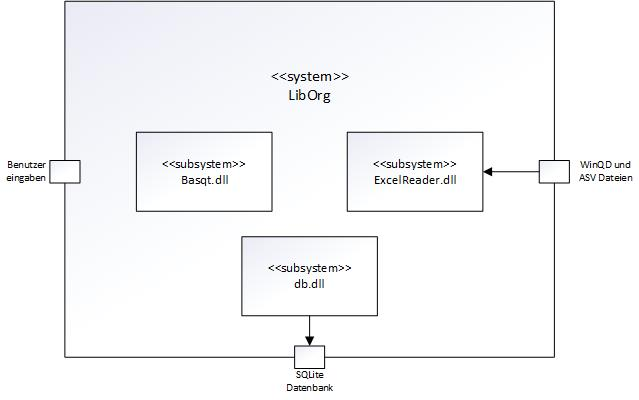
\includegraphics[width=0.60\textwidth]{figures/Bausteinschicht.jpg}
	\caption{LibOrg, Bausteinsicht}
	\label{fig:Bausteinsicht}
\end{figure}  
\begin{table}[H]
\begin{tabular}{|l|l|}
\hline
Modul           & Kurzbeschreibung                                                                                                                    \\ \hline
db.dll          & Realisiert die Kommunikation und den Datenaustausch mit der Datenbank.                                                              \\ \hline
ExcelReader.dll & Beinhaltet die Funktionalität, zum Import der Schülerdaten aus den  \\
				& ASV- und WinQD-Dateien\\ \hline
baseqt.dll      & Enthält einige grundlegende Funktionen der Anwendung, darunter den About- und  \\ 
				& den Settingsdialog und die Funktionalität der Config. \\ \hline
LibOrg          & Die eigentliche Hauptanwendung, dient zum Verwalten der Schüler und Bücherdaten.  \\  
				& Sowie die Ausleihen und Rückgaben der Bücher. \\ \hline 
\end{tabular}
\end{table}


\subsection{Db.dll}
\subsubsection{Zweck}
Dieses Modul realisiert die Kommunikation mit der Datenbank. Hierzu stellt es alle 
benötigten Funktionen bereit, um Daten in die Datenbank zu schreiben und auszulesen. 
Dafür wird eine Funktion des Moduls von der Hauptanwendung mit den erforderlichen 
Daten aufgerufen. Diese Funktion formatiert die Daten als funktionsfähiges SQL Statement
und ruft dieses auf der SQLite Datenbank auf. Dadurch wird die Integrität der Datenbank 
sichergestellt. Zusätzlich zu dieser Datenbank API, enthält die db.dll außerdem noch den 
Importdialog des ExcelReaders, die Funktionalität für das Datenbankbackup und den Logindialog.  
\subsubsection{Wichtige Funktionen}
\begin{figure}[H]
	\centering
		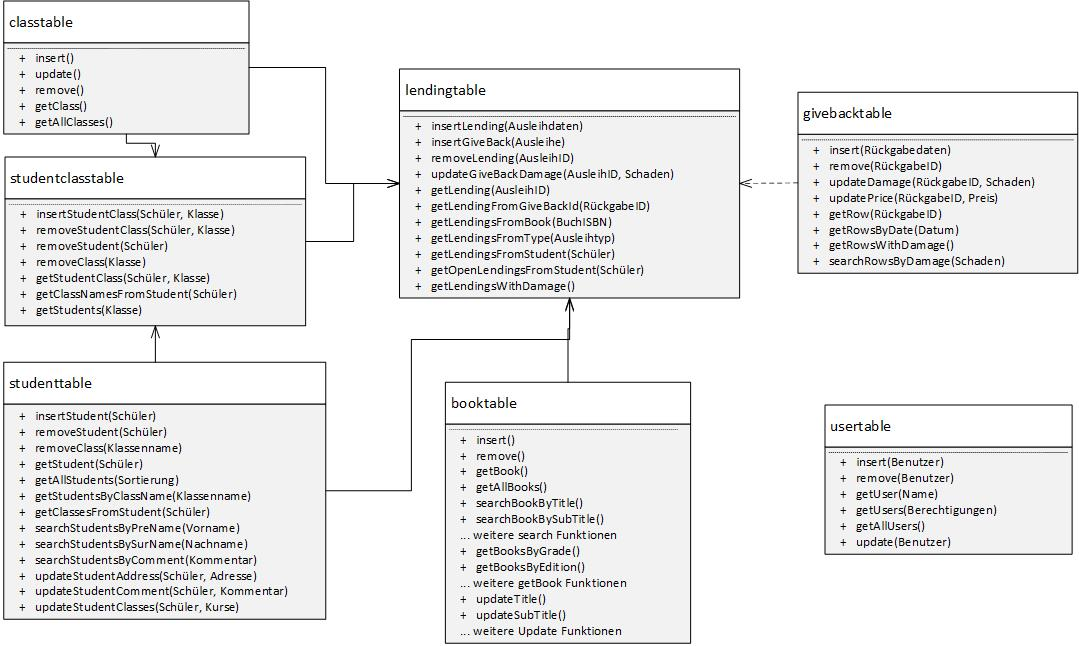
\includegraphics[width=0.95\textwidth]{figures/dbDLL.jpg}
	\caption{Überblick über die wichtigsten Funktionen der Datenbank API}
	\label{fig:dbDLL}
\end{figure}
\subsubsection{Ablageort/Datei}
Die Implementierung liegt unterhalb von Source.db.
\subsubsection{Offene Punkte}
Die Implemntierung dieses Datenbankinterfaces ist genau auf die Verwendung mit LibOrg
zugeschnitten, daher gibt es keine offenen Punkte. Allerdings muss das Interface bei 
Verwendung mit einer anderen Anwendung angepasst werden.


\subsection{ExcelReader.dll}
\subsubsection{Zweck}
Dieses Modul realisiert den Import der Schülerdaten zu Beginn des Schuljahres. Dafür 
liest es die verfügbaren Daten aus den WinQD- und ASV-Dateien aus. Bei diesen Dateien
handelt es sich um Daten in Tabellenform. Das Programm interpretiert die Daten, schreibt
die benötigten in die Datenbank und verwirft die überflüssigen. Natürlich setzt der 
ExcelReader voraus, dass die Formatierung der Dateien immer gleich vorliegt. Ebenso 
stellt er eine Fehlererkennung mit einer detailierten Ausgabe der, während des Imports
aufgetretenen, Fehler bereit.    
\subsubsection{Wichtige Funktionen}
\begin{figure}[H]
	\centering
		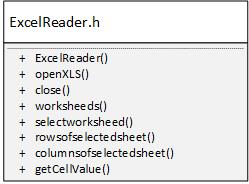
\includegraphics[width=0.30\textwidth]{figures/ExcelReader.jpg}
	\caption{Überblick über die wichtigsten Funktionen des ExcelReaders}
	\label{fig:ExcelReader}
\end{figure}
\subsubsection{Ablageort/Datei}
Die Implementierung liegt unterhalb von Source.ExcelReader.
\subsubsection{Offene Punkte}
Der ExcelReader ist vollständig Implementiert, jedoch könnte zur Erhöhung der Benutzerfreundlichkeit, noch eine direkte Fehlerbehandlung hinzugefügt werden.


\subsection{Baseqt.dll}
\subsubsection{Zweck}
Dieses Modul realisiert einige grundlegende Funktionen, welche zwar für das
Programm nötig sind, sich aber von den Grundfunktionalitäten trennen lassen. 
Daher können diese Funktionen in eine DLL ausgelagert werden. Zu diesen 
Funktionalitäten gehören:
\begin{enumerate}
\item{Überdialog}\\
	Ein Dialog, welcher Informationen über das Programm gibt, z.B. welche Version
	momentan installiert ist.
\item{Base Excpetion}\\
	Eine grunglegende Funktion um Exceptions, mit ErrorCode und Erklärung, zu verarbeiten.
\item{Konfiguration}\\
	Stellt die Funktionalität bereit, um grunglegende Einstellungen in einer Config-Datei
	zu speichern und danach zu laden.
\item{Lizenzplugin}\\
	Ein Dialog, welcher die GPL-Lizenz anzeigt, um auf die Verwendung dieser Lizenz hinzuweisen.
\item{Einstellungsdialog}\\
	Ein Dialog, um die grundlegenden Einstellung zu bearbeiten. Diese Einstellungen werden dann
	in der Konfigurationsdatei gespeichert.
\end{enumerate} 
\subsubsection{Wichtige Funktionen}
\begin{figure}[H]
	\centering
		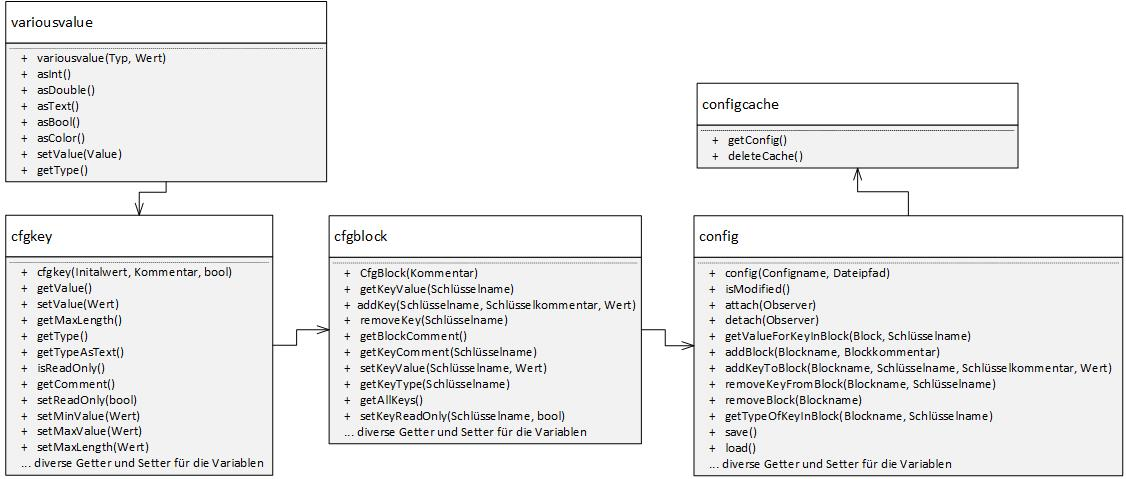
\includegraphics[width=0.95\textwidth]{figures/baseqt.jpg}
	\caption{Überblick über die wichtigsten Funktionen der Config in baseqt}
	\label{fig:baseqt}
\end{figure}
\subsubsection{Ablageort/Datei}
Die Implementierung liegt unterhalb von Source.baseqt.
\subsubsection{Offene Punkte}
Die Implementierung ist im Rahmen des Programms vollständig.


\subsection{Hauptanwendung LibOrg}
\subsubsection{Zweck}
Dieses Modul realisiert die Hauptanwendung der Software, daher stellt es alle Funktionen 
bereit, um Schüler und Bücher hinzuzufügen, zu bearbeiten oder zu löschen. Zusätzlich 
werden hier die Ausleihe- und Rückgabevorgänge abgebildet. Ebenso wird das GUI hier 
verwaltet und initalisiert. Dieses Modul enthält die Main-Funktion.
\subsubsection{Wichtige Funktionen}
\begin{figure}[H]
	\centering
		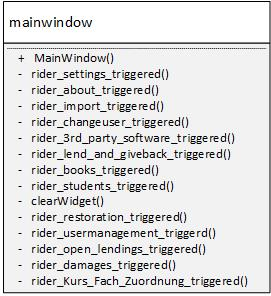
\includegraphics[width=0.20\textwidth]{figures/Mainwindow.jpg}
	\caption{Überblick über die Slots des Mainwindows }
	\label{fig:LibOrg}
\end{figure}

\subsubsection{Ablageort/Datei}
Die Implementierung liegt unterhalb von Sourc.MainProject.
\subsubsection{Offene Punkte}
Da es sich hierbei um die Hauptanwendung handelt, muss dieses Modul, für jedes neue Feature,
abgeändert werden. Für den Realesstand 1.0 ist die Implementierung vollständig.